\newif\ifsolutions
\solutionstrue % Show solutions
%\solutionsfalse % Hide solutions

\documentclass{article}
\usepackage{geometry}
\geometry{margin=1in}
\usepackage{tikz}
\usepackage{amssymb}

% fleqn allows setting indent of display math
\usepackage[fleqn]{amsmath}
\setlength{\mathindent}{0pt} % Set indent
% Disable equation numbering (https://tex.stackexchange.com/a/360378)
\makeatletter
\renewcommand\tagform@[1]{}
\makeatother

% Allow Unicode (some, e.g., © and £ at least)
% https://tex.stackexchange.com/questions/370278/is-there-any-reason-to-use-inputenc
\usepackage[utf8]{inputenc}

% Hyperlinks
\usepackage{hyperref}
\hypersetup{colorlinks=true, urlcolor=blue, linkcolor=blue}

% Prevent indentation of paragraphs
\setlength\parindent{0pt}
\setlength{\parskip}{\baselineskip}

% Spacing above/below equations
% https://tex.stackexchange.com/a/69678
\AtBeginDocument{%
 \abovedisplayskip=-\parskip
 \abovedisplayshortskip=-\parskip
 \belowdisplayskip=-\parskip
 \belowdisplayshortskip=-\parskip
}

% Allow 3 additional subsection levels
% https://tex.stackexchange.com/a/60212
\usepackage{titlesec}
\setcounter{secnumdepth}{6}
% H4 in HTML
\titleformat{\paragraph}{\normalfont\normalsize\bfseries}{\theparagraph}{1em}{}
\titlespacing*{\paragraph}{0pt}{3.25ex plus 1ex minus .2ex}{1.5ex plus .2ex}
% H5 in HTML
\titleformat{\subparagraph}{\normalfont\normalsize\bfseries}{\thesubparagraph}{1em}{}
\titlespacing*{\subparagraph}{0pt}{3.25ex plus 1ex minus .2ex}{1.5ex plus .2ex}
% H6 in HTML
\titleformat{\subsubparagraph}{\normalfont\normalsize\bfseries}{\thesubsubparagraph}{1em}{}
\titlespacing*{\subsubparagraph}{0pt}{3.25ex plus 1ex minus .2ex}{1.5ex plus .2ex}

\renewcommand{\mbox}{\text}
\newcommand{\ds}[0]{\displaystyle}
\newcommand{\ihat}[0]{\hat{\boldsymbol{\imath}}}
\newcommand{\jhat}[0]{\hat{\boldsymbol{\jmath}}}
\newcommand{\khat}[0]{\hat{\boldsymbol{k}}}
\newcommand{\xhat}[0]{\hat{\mathbf{x}}}
\newcommand{\yhat}[0]{\hat{\mathbf{y}}}
\newcommand{\zhat}[0]{\hat{\mathbf{z}}}
\newcommand{\rhat}[0]{\hat{\mathbf{r}}}
\newcommand{\bfvec}[1]{\vec{\mathbf{#1}}}
\newcommand{\bfcdot}[0]{\boldsymbol{\cdot}}

\usepackage{fancyhdr}
\pagestyle{fancy}
\lhead{Enclosed Charge}
\rhead{\thepage}
\fancyfoot{}

\begin{document}

\section{Overview}

When using Gauss's law, one must draw an imaginary volume in space and compute how much charge is inside the volume.

In general, an imaginary volume is chosen is one for which computation of the electric flux is easy. That is, the imaginary volume will be such that the electric field is either parallel or perpendicular to all parts of the surface. In this activity, you are given the Gaussian volume. However, you should understand the reason for the choice of each Gaussian volume given.

\section{Line of Charge}

A total of $+3Q$ is uniformly distributed a non--conducting line of length $L$. The Gaussian cylinder shown has a length $h$, radius $r$, and the same center line as the charged line.



\tikzset{every picture/.style={line width=0.75pt}} %set default line width to 0.75pt        

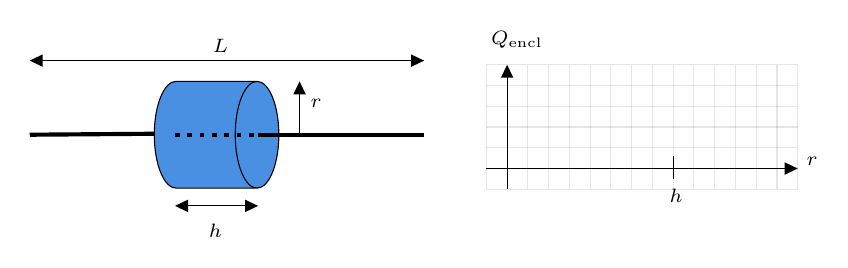
\begin{tikzpicture}[x=0.75pt,y=0.75pt,yscale=-1,xscale=1]
%uncomment if require: \path (0,113); %set diagram left start at 0, and has height of 113

%Flowchart: Direct Access Storage [id:dp2523632931053985] 
\draw  [fill={rgb, 255:red, 74; green, 144; blue, 226 }  ,fill opacity=1 ] (129.5,79.43) -- (90.5,79.43) .. controls (84.7,79.43) and (80,67.92) .. (80,53.71) .. controls (80,39.51) and (84.7,28) .. (90.5,28) -- (129.5,28)(140,53.71) .. controls (140,67.92) and (135.3,79.43) .. (129.5,79.43) .. controls (123.7,79.43) and (119,67.92) .. (119,53.71) .. controls (119,39.51) and (123.7,28) .. (129.5,28) .. controls (135.3,28) and (140,39.51) .. (140,53.71) ;
%Straight Lines [id:da2128877957194073] 
\draw [line width=1.5]    (20,53.71) -- (80,53.24) ;
%Straight Lines [id:da8973887652942925] 
\draw [line width=1.5]    (130,53.71) -- (210,53.71) ;
%Straight Lines [id:da09343418673905979] 
\draw [line width=1.5]  [dash pattern={on 1.69pt off 2.76pt}]  (90,53.71) -- (130,53.71) ;
%Shape: Grid [id:dp9875189635012225] 
\draw  [draw opacity=0] (240,20) -- (390,20) -- (390,80) -- (240,80) -- cycle ; \draw  [color={rgb, 255:red, 0; green, 0; blue, 0 }  ,draw opacity=0.1 ] (240,20) -- (240,80)(250,20) -- (250,80)(260,20) -- (260,80)(270,20) -- (270,80)(280,20) -- (280,80)(290,20) -- (290,80)(300,20) -- (300,80)(310,20) -- (310,80)(320,20) -- (320,80)(330,20) -- (330,80)(340,20) -- (340,80)(350,20) -- (350,80)(360,20) -- (360,80)(370,20) -- (370,80)(380,20) -- (380,80) ; \draw  [color={rgb, 255:red, 0; green, 0; blue, 0 }  ,draw opacity=0.1 ] (240,20) -- (390,20)(240,30) -- (390,30)(240,40) -- (390,40)(240,50) -- (390,50)(240,60) -- (390,60)(240,70) -- (390,70) ; \draw  [color={rgb, 255:red, 0; green, 0; blue, 0 }  ,draw opacity=0.1 ]  ;
%Straight Lines [id:da9734706800390553] 
\draw [color={rgb, 255:red, 0; green, 0; blue, 0 }  ,draw opacity=0.1 ]   (240,80) -- (390,80) ;
%Straight Lines [id:da6432884490747786] 
\draw [color={rgb, 255:red, 0; green, 0; blue, 0 }  ,draw opacity=0.1 ]   (390,80) -- (390,20) ;

%Straight Lines [id:da029072803872031594] 
\draw    (250,23) -- (250,80) ;
\draw [shift={(250,20)}, rotate = 90] [fill={rgb, 255:red, 0; green, 0; blue, 0 }  ][line width=0.08]  [draw opacity=0] (6.25,-3) -- (0,0) -- (6.25,3) -- cycle    ;
%Straight Lines [id:da733891856041468] 
\draw    (240,70) -- (387,70) ;
\draw [shift={(390,70)}, rotate = 180] [fill={rgb, 255:red, 0; green, 0; blue, 0 }  ][line width=0.08]  [draw opacity=0] (6.25,-3) -- (0,0) -- (6.25,3) -- cycle    ;
%Straight Lines [id:da5848925936939344] 
\draw    (330,64) -- (330,75) ;
%Straight Lines [id:da6508968321800463] 
\draw    (93,88) -- (127,88) ;
\draw [shift={(130,88)}, rotate = 180] [fill={rgb, 255:red, 0; green, 0; blue, 0 }  ][line width=0.08]  [draw opacity=0] (6.25,-3) -- (0,0) -- (6.25,3) -- cycle    ;
\draw [shift={(90,88)}, rotate = 0] [fill={rgb, 255:red, 0; green, 0; blue, 0 }  ][line width=0.08]  [draw opacity=0] (6.25,-3) -- (0,0) -- (6.25,3) -- cycle    ;
%Straight Lines [id:da9876972360001792] 
\draw    (150,53.71) -- (150,31) ;
\draw [shift={(150,28)}, rotate = 90] [fill={rgb, 255:red, 0; green, 0; blue, 0 }  ][line width=0.08]  [draw opacity=0] (6.25,-3) -- (0,0) -- (6.25,3) -- cycle    ;
%Straight Lines [id:da893064176898352] 
\draw    (23,18) -- (207,18) ;
\draw [shift={(210,18)}, rotate = 180] [fill={rgb, 255:red, 0; green, 0; blue, 0 }  ][line width=0.08]  [draw opacity=0] (6.25,-3) -- (0,0) -- (6.25,3) -- cycle    ;
\draw [shift={(20,18)}, rotate = 0] [fill={rgb, 255:red, 0; green, 0; blue, 0 }  ][line width=0.08]  [draw opacity=0] (6.25,-3) -- (0,0) -- (6.25,3) -- cycle    ;

% Text Node
\draw (241,2.4) node [anchor=north west][inner sep=0.75pt]  [font=\scriptsize]  {$Q\mathrm{_{encl}}$};
% Text Node
\draw (393,63.4) node [anchor=north west][inner sep=0.75pt]  [font=\scriptsize]  {$r$};
% Text Node
\draw (327,78.4) node [anchor=north west][inner sep=0.75pt]  [font=\scriptsize]  {$h$};
% Text Node
\draw (105,95.4) node [anchor=north west][inner sep=0.75pt]  [font=\scriptsize]  {$h$};
% Text Node
\draw (154,35.4) node [anchor=north west][inner sep=0.75pt]  [font=\scriptsize]  {$r$};
% Text Node
\draw (107,6.4) node [anchor=north west][inner sep=0.75pt]  [font=\scriptsize]  {$L$};


\end{tikzpicture}


\begin{enumerate}

  \item Find the linear charge density, $\lambda$, on the line.

        \ifsolutions
          \textbf{Answer}: The linear charge density is the total charge divided by the length over which the charge is distributed: $\lambda={3Q}/{L}$.
        \else
          \vskip 36.135pt
        \fi

  \item Find an equation for $Q_{\text{encl}}$ in terms of $\lambda$ and one or more of $r$, $h$, and $L$.

        \ifsolutions
          \textbf{Answer}: The dashed line in the figure is the part of the line inside of the Gaussian cylinder. The length of the dashed line is $h$, so $Q_{\text{encl}}=\lambda h$. Another way of arriving at this is by noting that the charge enclosed is the total charge $\times$ the ratio $h/L$, so $Q_{\text{encl}}=3Q(h/L) = \lambda h$.
        \else
          \vskip 36.135pt
        \fi

  \item Use your equation from 2. to find the amount of charge enclosed by the Gaussian cylinder when it has radii of $r=h/100$, $r=h/2$, $r=h$, and $r=2h$.

        \ifsolutions
          \textbf{Answer}: $Q_{\text{encl}}=\lambda h$ for all four cases.
        \else
          \vskip 36.135pt
        \fi

  \item Plot the four values of enclosed charge calculated above versus the radius of the Gaussian cylinder. Then plot the equation found in part 2. as a smooth line.

        \ifsolutions
          \textbf{Answer:}
        
          

\tikzset{every picture/.style={line width=0.75pt}} %set default line width to 0.75pt        

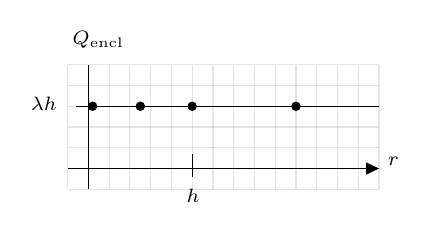
\begin{tikzpicture}[x=0.75pt,y=0.75pt,yscale=-1,xscale=1]
%uncomment if require: \path (0,95); %set diagram left start at 0, and has height of 95

%Shape: Grid [id:dp10908942556051615] 
\draw  [draw opacity=0] (20,20) -- (170,20) -- (170,80) -- (20,80) -- cycle ; \draw  [color={rgb, 255:red, 0; green, 0; blue, 0 }  ,draw opacity=0.1 ] (20,20) -- (20,80)(30,20) -- (30,80)(40,20) -- (40,80)(50,20) -- (50,80)(60,20) -- (60,80)(70,20) -- (70,80)(80,20) -- (80,80)(90,20) -- (90,80)(100,20) -- (100,80)(110,20) -- (110,80)(120,20) -- (120,80)(130,20) -- (130,80)(140,20) -- (140,80)(150,20) -- (150,80)(160,20) -- (160,80) ; \draw  [color={rgb, 255:red, 0; green, 0; blue, 0 }  ,draw opacity=0.1 ] (20,20) -- (170,20)(20,30) -- (170,30)(20,40) -- (170,40)(20,50) -- (170,50)(20,60) -- (170,60)(20,70) -- (170,70) ; \draw  [color={rgb, 255:red, 0; green, 0; blue, 0 }  ,draw opacity=0.1 ]  ;
%Straight Lines [id:da5793514725444062] 
\draw [color={rgb, 255:red, 0; green, 0; blue, 0 }  ,draw opacity=0.1 ]   (20,80) -- (170,80) ;
%Straight Lines [id:da020612542975321224] 
\draw [color={rgb, 255:red, 0; green, 0; blue, 0 }  ,draw opacity=0.1 ]   (170,80) -- (170,20) ;

%Straight Lines [id:da26265464079120404] 
\draw    (30,20) -- (30,80) ;
%Straight Lines [id:da25909733967204973] 
\draw    (20,70) -- (167,70) ;
\draw [shift={(170,70)}, rotate = 180] [fill={rgb, 255:red, 0; green, 0; blue, 0 }  ][line width=0.08]  [draw opacity=0] (6.25,-3) -- (0,0) -- (6.25,3) -- cycle    ;
%Shape: Circle [id:dp44641273614521926] 
\draw  [fill={rgb, 255:red, 0; green, 0; blue, 0 }  ,fill opacity=1 ] (30,40) .. controls (30,38.9) and (30.9,38) .. (32,38) .. controls (33.1,38) and (34,38.9) .. (34,40) .. controls (34,41.1) and (33.1,42) .. (32,42) .. controls (30.9,42) and (30,41.1) .. (30,40) -- cycle ;
%Shape: Circle [id:dp3120297789520805] 
\draw  [fill={rgb, 255:red, 0; green, 0; blue, 0 }  ,fill opacity=1 ] (53,40) .. controls (53,38.9) and (53.9,38) .. (55,38) .. controls (56.1,38) and (57,38.9) .. (57,40) .. controls (57,41.1) and (56.1,42) .. (55,42) .. controls (53.9,42) and (53,41.1) .. (53,40) -- cycle ;
%Shape: Circle [id:dp5784910284605251] 
\draw  [fill={rgb, 255:red, 0; green, 0; blue, 0 }  ,fill opacity=1 ] (78,40) .. controls (78,38.9) and (78.9,38) .. (80,38) .. controls (81.1,38) and (82,38.9) .. (82,40) .. controls (82,41.1) and (81.1,42) .. (80,42) .. controls (78.9,42) and (78,41.1) .. (78,40) -- cycle ;
%Shape: Circle [id:dp6567841873311164] 
\draw  [fill={rgb, 255:red, 0; green, 0; blue, 0 }  ,fill opacity=1 ] (128,40) .. controls (128,38.9) and (128.9,38) .. (130,38) .. controls (131.1,38) and (132,38.9) .. (132,40) .. controls (132,41.1) and (131.1,42) .. (130,42) .. controls (128.9,42) and (128,41.1) .. (128,40) -- cycle ;
%Straight Lines [id:da9640426388934846] 
\draw    (80,63) -- (80,74) ;
%Straight Lines [id:da02907769084038314] 
\draw    (24,40) -- (34,40) ;
%Straight Lines [id:da9479293837523952] 
\draw    (34,40) -- (170,40) ;

% Text Node
\draw (21,2.4) node [anchor=north west][inner sep=0.75pt]  [font=\scriptsize]  {$Q\mathrm{_{encl}}$};
% Text Node
\draw (173,63.4) node [anchor=north west][inner sep=0.75pt]  [font=\scriptsize]  {$r$};
% Text Node
\draw (76,78.4) node [anchor=north west][inner sep=0.75pt]  [font=\scriptsize]  {$h$};
% Text Node
\draw (1,34.4) node [anchor=north west][inner sep=0.75pt]  [font=\scriptsize]  {$\lambda h$};


\end{tikzpicture}

        \else
          \newpage
        \fi

\end{enumerate}

\section{Cylindrical Shell}

A non--conducting hollow cylinder of radius $R$ and length $H$ has a charge of $+3Q$ uniformly distributed on its curved surface. The Gaussian cylinder shown has a length $h$, radius $r$, and the same center line as the charged cylinder.



\tikzset{every picture/.style={line width=0.75pt}} %set default line width to 0.75pt        

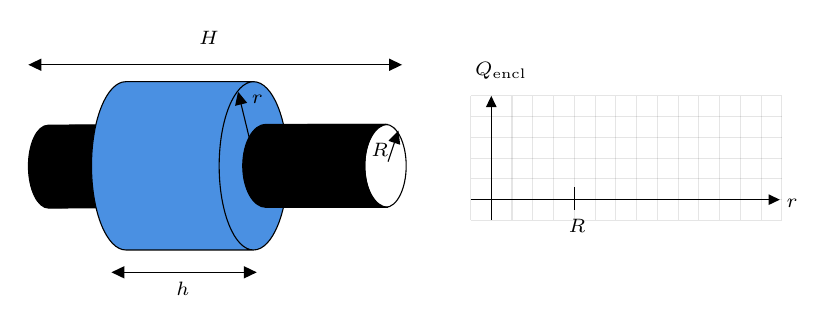
\begin{tikzpicture}[x=0.75pt,y=0.75pt,yscale=-1,xscale=1]
%uncomment if require: \path (0,143); %set diagram left start at 0, and has height of 143

%Flowchart: Stored Data [id:dp6886906265148047] 
\draw  [fill={rgb, 255:red, 0; green, 0; blue, 0 }  ,fill opacity=1 ] (16.42,54.14) -- (66.82,53.69) .. controls (61.52,53.74) and (57.3,62.72) .. (57.4,73.74) .. controls (57.5,84.77) and (61.87,93.67) .. (67.17,93.62) -- (16.78,94.07) .. controls (11.48,94.11) and (7.1,85.22) .. (7,74.19) .. controls (6.9,63.17) and (11.12,54.19) .. (16.42,54.14) -- cycle ;
%Flowchart: Direct Access Storage [id:dp6433796594195302] 
\draw  [fill={rgb, 255:red, 74; green, 144; blue, 226 }  ,fill opacity=1 ] (115.44,114.24) -- (53.95,114.24) .. controls (44.8,114.24) and (37.39,96.09) .. (37.39,73.69) .. controls (37.39,51.3) and (44.8,33.15) .. (53.95,33.15) -- (115.44,33.15)(132,73.69) .. controls (132,96.09) and (124.58,114.24) .. (115.44,114.24) .. controls (106.3,114.24) and (98.89,96.09) .. (98.89,73.69) .. controls (98.89,51.3) and (106.3,33.15) .. (115.44,33.15) .. controls (124.58,33.15) and (132,51.3) .. (132,73.69) ;
%Flowchart: Direct Access Storage [id:dp43794934680039765] 
\draw   (179.02,93.69) -- (141.97,93.69) .. controls (136.46,93.69) and (132,84.74) .. (132,73.69) .. controls (132,62.65) and (136.46,53.69) .. (141.97,53.69) -- (179.02,53.69)(189,73.69) .. controls (189,84.74) and (184.53,93.69) .. (179.02,93.69) .. controls (173.51,93.69) and (169.05,84.74) .. (169.05,73.69) .. controls (169.05,62.65) and (173.51,53.69) .. (179.02,53.69) .. controls (184.53,53.69) and (189,62.65) .. (189,73.69) ;
%Flowchart: Stored Data [id:dp38629361535592754] 
\draw  [fill={rgb, 255:red, 0; green, 0; blue, 0 }  ,fill opacity=1 ] (121.45,53.69) -- (180.25,53.69) .. controls (174.06,53.69) and (169.05,62.65) .. (169.05,73.69) .. controls (169.05,84.74) and (174.06,93.69) .. (180.25,93.69) -- (121.45,93.69) .. controls (115.26,93.69) and (110.25,84.74) .. (110.25,73.69) .. controls (110.25,62.65) and (115.26,53.69) .. (121.45,53.69) -- cycle ;
%Straight Lines [id:da12895551872078115] 
\draw    (50,125) -- (114,125) ;
\draw [shift={(117,125)}, rotate = 180] [fill={rgb, 255:red, 0; green, 0; blue, 0 }  ][line width=0.08]  [draw opacity=0] (6.25,-3) -- (0,0) -- (6.25,3) -- cycle    ;
\draw [shift={(47,125)}, rotate = 0] [fill={rgb, 255:red, 0; green, 0; blue, 0 }  ][line width=0.08]  [draw opacity=0] (6.25,-3) -- (0,0) -- (6.25,3) -- cycle    ;
%Straight Lines [id:da8425966711715258] 
\draw    (10,25) -- (184,25) ;
\draw [shift={(187,25)}, rotate = 180] [fill={rgb, 255:red, 0; green, 0; blue, 0 }  ][line width=0.08]  [draw opacity=0] (6.25,-3) -- (0,0) -- (6.25,3) -- cycle    ;
\draw [shift={(7,25)}, rotate = 0] [fill={rgb, 255:red, 0; green, 0; blue, 0 }  ][line width=0.08]  [draw opacity=0] (6.25,-3) -- (0,0) -- (6.25,3) -- cycle    ;
%Straight Lines [id:da8187795038897792] 
\draw    (180.25,71.69) -- (184.3,59.54) ;
\draw [shift={(185.25,56.69)}, rotate = 108.43] [fill={rgb, 255:red, 0; green, 0; blue, 0 }  ][line width=0.08]  [draw opacity=0] (6.25,-3) -- (0,0) -- (6.25,3) -- cycle    ;
%Straight Lines [id:da8286231758044365] 
\draw    (108.71,40.92) -- (116.29,72.08) ;
\draw [shift={(117,75)}, rotate = 256.33] [fill={rgb, 255:red, 0; green, 0; blue, 0 }  ][line width=0.08]  [draw opacity=0] (6.25,-3) -- (0,0) -- (6.25,3) -- cycle    ;
\draw [shift={(108,38)}, rotate = 76.33] [fill={rgb, 255:red, 0; green, 0; blue, 0 }  ][line width=0.08]  [draw opacity=0] (6.25,-3) -- (0,0) -- (6.25,3) -- cycle    ;
%Shape: Grid [id:dp8669847375163626] 
\draw  [draw opacity=0] (220,40) -- (370,40) -- (370,100) -- (220,100) -- cycle ; \draw  [color={rgb, 255:red, 0; green, 0; blue, 0 }  ,draw opacity=0.1 ] (220,40) -- (220,100)(230,40) -- (230,100)(240,40) -- (240,100)(250,40) -- (250,100)(260,40) -- (260,100)(270,40) -- (270,100)(280,40) -- (280,100)(290,40) -- (290,100)(300,40) -- (300,100)(310,40) -- (310,100)(320,40) -- (320,100)(330,40) -- (330,100)(340,40) -- (340,100)(350,40) -- (350,100)(360,40) -- (360,100) ; \draw  [color={rgb, 255:red, 0; green, 0; blue, 0 }  ,draw opacity=0.1 ] (220,40) -- (370,40)(220,50) -- (370,50)(220,60) -- (370,60)(220,70) -- (370,70)(220,80) -- (370,80)(220,90) -- (370,90) ; \draw  [color={rgb, 255:red, 0; green, 0; blue, 0 }  ,draw opacity=0.1 ]  ;
%Straight Lines [id:da9988647785859446] 
\draw [color={rgb, 255:red, 0; green, 0; blue, 0 }  ,draw opacity=0.1 ]   (220,100) -- (370,100) ;
%Straight Lines [id:da8444762203883653] 
\draw [color={rgb, 255:red, 0; green, 0; blue, 0 }  ,draw opacity=0.1 ]   (370,100) -- (370,40) ;

%Straight Lines [id:da2300204175853655] 
\draw    (230,43) -- (230,100) ;
\draw [shift={(230,40)}, rotate = 90] [fill={rgb, 255:red, 0; green, 0; blue, 0 }  ][line width=0.08]  [draw opacity=0] (5.36,-2.57) -- (0,0) -- (5.36,2.57) -- cycle    ;
%Straight Lines [id:da8858475685329994] 
\draw [color={rgb, 255:red, 0; green, 0; blue, 0 }  ,draw opacity=1 ]   (220,90) -- (366,90) ;
\draw [shift={(369,90)}, rotate = 180] [fill={rgb, 255:red, 0; green, 0; blue, 0 }  ,fill opacity=1 ][line width=0.08]  [draw opacity=0] (5.36,-2.57) -- (0,0) -- (5.36,2.57) -- cycle    ;
%Straight Lines [id:da0010120684278946968] 
\draw    (270,84) -- (270,95) ;

% Text Node
\draw (77,128.4) node [anchor=north west][inner sep=0.75pt]  [font=\scriptsize]  {$h$};
% Text Node
\draw (88,7.4) node [anchor=north west][inner sep=0.75pt]  [font=\scriptsize]  {$H$};
% Text Node
\draw (171,61.4) node [anchor=north west][inner sep=0.75pt]  [font=\scriptsize]  {$R$};
% Text Node
\draw (113.44,38.55) node [anchor=north west][inner sep=0.75pt]  [font=\scriptsize]  {$r$};
% Text Node
\draw (221,22.4) node [anchor=north west][inner sep=0.75pt]  [font=\scriptsize]  {$Q_{\mathrm{encl}}$};
% Text Node
\draw (266,98.4) node [anchor=north west][inner sep=0.75pt]  [font=\scriptsize]  {$R$};
% Text Node
\draw (371,88.4) node [anchor=north west][inner sep=0.75pt]  [font=\scriptsize]  {$r$};


\end{tikzpicture}


\begin{enumerate}

  \item Find the linear charge density, $\lambda$, of the charged cylinder.

        \ifsolutions
          \textbf{Answer}: The linear charge density is the total charge divided by the length over which the charge is distributed: $\lambda={3Q}/{H}$.
        
          \textbf{Note}: The charges are distributed on a surface, so it may seem more natural to use a surface charge density, which is $\sigma = 3Q/(2\pi R H)$, where the denominator is the surface area of the curved part of the charged cylinder. In this case, the answer to 2. does not change and the answer to 3. is $Q_{\text{encl}} = \sigma 2\pi R h$ instead of $Q_{\text{encl}}=\lambda h$. We use charge per length in this problem because the formula for $Q_{\text{encl}}$ is simpler.
        \else
          \vskip 36.135pt
        \fi

  \item Find an equation for $Q_{\text{encl}}$ for $r<R$.

        \ifsolutions
          \textbf{Answer}: If the Gaussian cylinder is fully inside the hollow cylinder, there would be no charge inside of it. As a result, the charge enclosed for $r< R$ is zero: $Q_{\text{encl}}=0$.
        \else
          \vskip 36.135pt
        \fi

  \item Find an equation for $Q_{\text{encl}}$ for $r>R$. Your equation should involve $\lambda$ and one or more of $h$, $r$, and $R$.

        \textbf{Answer}: The amount of charge enclosed is the charge per unit length $\times h = \lambda h$, so  $Q_{\text{encl}}=\lambda h$. (The amount of charge enclosed does not depend on $r$.)

        \ifsolutions\else
        \vskip 36.135pt
        \fi

  \item Find the amount of charge enclosed by the Gaussian cylinder when it has radii of $r=0$, $r=R/2$, $r=2R$, and $r=3R$.

        \ifsolutions
          \textbf{Answer}: $0, 0, \lambda h, \lambda h$
        \else
          \vskip 36.135pt
        \fi

  \item Plot the four values of enclosed charge calculated above versus the radius of the Gaussian cylinder. Then plot the equations found in parts 2. and 3 as a smooth line.

        \ifsolutions
          

\tikzset{every picture/.style={line width=0.75pt}} %set default line width to 0.75pt        

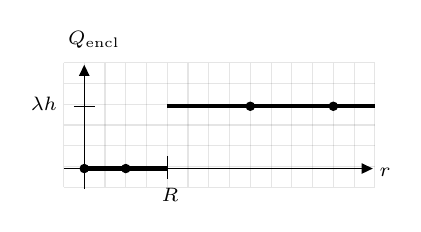
\begin{tikzpicture}[x=0.75pt,y=0.75pt,yscale=-1,xscale=1]
%uncomment if require: \path (0,94); %set diagram left start at 0, and has height of 94

%Shape: Grid [id:dp4595545900919136] 
\draw  [draw opacity=0] (20,20) -- (170,20) -- (170,80) -- (20,80) -- cycle ; \draw  [color={rgb, 255:red, 0; green, 0; blue, 0 }  ,draw opacity=0.1 ] (20,20) -- (20,80)(30,20) -- (30,80)(40,20) -- (40,80)(50,20) -- (50,80)(60,20) -- (60,80)(70,20) -- (70,80)(80,20) -- (80,80)(90,20) -- (90,80)(100,20) -- (100,80)(110,20) -- (110,80)(120,20) -- (120,80)(130,20) -- (130,80)(140,20) -- (140,80)(150,20) -- (150,80)(160,20) -- (160,80) ; \draw  [color={rgb, 255:red, 0; green, 0; blue, 0 }  ,draw opacity=0.1 ] (20,20) -- (170,20)(20,30) -- (170,30)(20,40) -- (170,40)(20,50) -- (170,50)(20,60) -- (170,60)(20,70) -- (170,70) ; \draw  [color={rgb, 255:red, 0; green, 0; blue, 0 }  ,draw opacity=0.1 ]  ;
%Straight Lines [id:da32569280071530327] 
\draw [color={rgb, 255:red, 0; green, 0; blue, 0 }  ,draw opacity=0.1 ]   (20,80) -- (170,80) ;
%Straight Lines [id:da591387116177337] 
\draw [color={rgb, 255:red, 0; green, 0; blue, 0 }  ,draw opacity=0.1 ]   (170,80) -- (170,20) ;

%Straight Lines [id:da12016986067225233] 
\draw    (30,24) -- (30,81) ;
\draw [shift={(30,21)}, rotate = 90] [fill={rgb, 255:red, 0; green, 0; blue, 0 }  ][line width=0.08]  [draw opacity=0] (5.36,-2.57) -- (0,0) -- (5.36,2.57) -- cycle    ;
%Straight Lines [id:da752832446770658] 
\draw [color={rgb, 255:red, 0; green, 0; blue, 0 }  ,draw opacity=1 ]   (20,71) -- (166,71) ;
\draw [shift={(169,71)}, rotate = 180] [fill={rgb, 255:red, 0; green, 0; blue, 0 }  ,fill opacity=1 ][line width=0.08]  [draw opacity=0] (5.36,-2.57) -- (0,0) -- (5.36,2.57) -- cycle    ;
%Shape: Circle [id:dp5679759155543898] 
\draw  [fill={rgb, 255:red, 0; green, 0; blue, 0 }  ,fill opacity=1 ] (28,71) .. controls (28,69.9) and (28.9,69) .. (30,69) .. controls (31.1,69) and (32,69.9) .. (32,71) .. controls (32,72.1) and (31.1,73) .. (30,73) .. controls (28.9,73) and (28,72.1) .. (28,71) -- cycle ;
%Shape: Circle [id:dp21558647180786772] 
\draw  [fill={rgb, 255:red, 0; green, 0; blue, 0 }  ,fill opacity=1 ] (48,71) .. controls (48,69.9) and (48.9,69) .. (50,69) .. controls (51.1,69) and (52,69.9) .. (52,71) .. controls (52,72.1) and (51.1,73) .. (50,73) .. controls (48.9,73) and (48,72.1) .. (48,71) -- cycle ;
%Shape: Circle [id:dp15640551520494061] 
\draw  [fill={rgb, 255:red, 0; green, 0; blue, 0 }  ,fill opacity=1 ] (108,41) .. controls (108,39.9) and (108.9,39) .. (110,39) .. controls (111.1,39) and (112,39.9) .. (112,41) .. controls (112,42.1) and (111.1,43) .. (110,43) .. controls (108.9,43) and (108,42.1) .. (108,41) -- cycle ;
%Shape: Circle [id:dp8505391806947797] 
\draw  [fill={rgb, 255:red, 0; green, 0; blue, 0 }  ,fill opacity=1 ] (148,41) .. controls (148,39.9) and (148.9,39) .. (150,39) .. controls (151.1,39) and (152,39.9) .. (152,41) .. controls (152,42.1) and (151.1,43) .. (150,43) .. controls (148.9,43) and (148,42.1) .. (148,41) -- cycle ;
%Straight Lines [id:da4664350184010533] 
\draw    (70,65) -- (70,76) ;
%Straight Lines [id:da48030994279797556] 
\draw    (25,41) -- (35,41) ;
%Straight Lines [id:da43441002194713496] 
\draw [line width=1.5]    (70,41) -- (170,41) ;
%Straight Lines [id:da5662828112090963] 
\draw [line width=1.5]    (32,71) -- (70,71) ;

% Text Node
\draw (21,3.4) node [anchor=north west][inner sep=0.75pt]  [font=\scriptsize]  {$Q_{\mathrm{encl}}$};
% Text Node
\draw (66,79.4) node [anchor=north west][inner sep=0.75pt]  [font=\scriptsize]  {$R$};
% Text Node
\draw (3,35.4) node [anchor=north west][inner sep=0.75pt]  [font=\scriptsize]  {$\lambda h$};
% Text Node
\draw (171,69.4) node [anchor=north west][inner sep=0.75pt]  [font=\scriptsize]  {$r$};


\end{tikzpicture}

        \fi

\end{enumerate}

\newpage

\section{Solid Cylinder}

A non--conducting solid cylinder of radius, $R$ and length, $L$ has a charge of $+3Q$ uniformly distributed throughout it. The Gaussian cylinder has length $h$, radius $r$, and the same center line as the charged cylinder.



\tikzset{every picture/.style={line width=0.75pt}} %set default line width to 0.75pt        

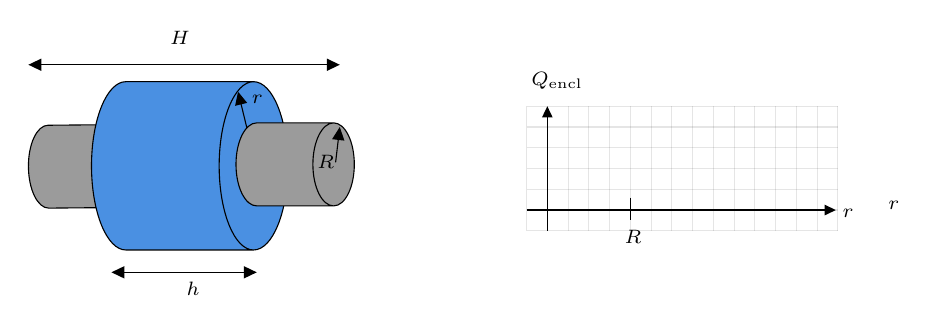
\begin{tikzpicture}[x=0.75pt,y=0.75pt,yscale=-1,xscale=1]
%uncomment if require: \path (0,150); %set diagram left start at 0, and has height of 150

%Flowchart: Stored Data [id:dp43279518290656416] 
\draw  [fill={rgb, 255:red, 155; green, 155; blue, 155 }  ,fill opacity=1 ] (29.42,59.14) -- (79.82,58.69) .. controls (74.52,58.74) and (70.3,67.72) .. (70.4,78.74) .. controls (70.5,89.77) and (74.87,98.67) .. (80.17,98.62) -- (29.78,99.07) .. controls (24.48,99.11) and (20.1,90.22) .. (20,79.19) .. controls (19.9,68.17) and (24.12,59.19) .. (29.42,59.14) -- cycle ;
%Flowchart: Direct Access Storage [id:dp644599832571805] 
\draw  [fill={rgb, 255:red, 74; green, 144; blue, 226 }  ,fill opacity=1 ] (128.44,119.24) -- (66.95,119.24) .. controls (57.8,119.24) and (50.39,101.09) .. (50.39,78.69) .. controls (50.39,56.3) and (57.8,38.15) .. (66.95,38.15) -- (128.44,38.15)(145,78.69) .. controls (145,101.09) and (137.58,119.24) .. (128.44,119.24) .. controls (119.3,119.24) and (111.89,101.09) .. (111.89,78.69) .. controls (111.89,56.3) and (119.3,38.15) .. (128.44,38.15) .. controls (137.58,38.15) and (145,56.3) .. (145,78.69) ;
%Shape: Grid [id:dp9022092561246653] 
\draw  [draw opacity=0] (260,50) -- (410,50) -- (410,110) -- (260,110) -- cycle ; \draw  [color={rgb, 255:red, 0; green, 0; blue, 0 }  ,draw opacity=0.1 ] (260,50) -- (260,110)(270,50) -- (270,110)(280,50) -- (280,110)(290,50) -- (290,110)(300,50) -- (300,110)(310,50) -- (310,110)(320,50) -- (320,110)(330,50) -- (330,110)(340,50) -- (340,110)(350,50) -- (350,110)(360,50) -- (360,110)(370,50) -- (370,110)(380,50) -- (380,110)(390,50) -- (390,110)(400,50) -- (400,110) ; \draw  [color={rgb, 255:red, 0; green, 0; blue, 0 }  ,draw opacity=0.1 ] (260,50) -- (410,50)(260,60) -- (410,60)(260,70) -- (410,70)(260,80) -- (410,80)(260,90) -- (410,90)(260,100) -- (410,100) ; \draw  [color={rgb, 255:red, 0; green, 0; blue, 0 }  ,draw opacity=0.1 ]  ;
%Straight Lines [id:da27282373130170723] 
\draw [color={rgb, 255:red, 0; green, 0; blue, 0 }  ,draw opacity=0.1 ]   (260,110) -- (410,110) ;
%Straight Lines [id:da4283303984115543] 
\draw [color={rgb, 255:red, 0; green, 0; blue, 0 }  ,draw opacity=0.1 ]   (410,110) -- (410,50) ;

%Straight Lines [id:da927798601778538] 
\draw    (270,53) -- (270,110) ;
\draw [shift={(270,50)}, rotate = 90] [fill={rgb, 255:red, 0; green, 0; blue, 0 }  ][line width=0.08]  [draw opacity=0] (5.36,-2.57) -- (0,0) -- (5.36,2.57) -- cycle    ;
%Straight Lines [id:da6159160274834647] 
\draw [color={rgb, 255:red, 0; green, 0; blue, 0 }  ,draw opacity=1 ]   (260,100) -- (406,100) ;
\draw [shift={(409,100)}, rotate = 180] [fill={rgb, 255:red, 0; green, 0; blue, 0 }  ,fill opacity=1 ][line width=0.08]  [draw opacity=0] (5.36,-2.57) -- (0,0) -- (5.36,2.57) -- cycle    ;
%Straight Lines [id:da4754703908366129] 
\draw    (310,94) -- (310,105) ;
%Straight Lines [id:da8177325762126639] 
\draw    (63,130) -- (127,130) ;
\draw [shift={(130,130)}, rotate = 180] [fill={rgb, 255:red, 0; green, 0; blue, 0 }  ][line width=0.08]  [draw opacity=0] (6.25,-3) -- (0,0) -- (6.25,3) -- cycle    ;
\draw [shift={(60,130)}, rotate = 0] [fill={rgb, 255:red, 0; green, 0; blue, 0 }  ][line width=0.08]  [draw opacity=0] (6.25,-3) -- (0,0) -- (6.25,3) -- cycle    ;
%Straight Lines [id:da359862491228339] 
\draw    (23,30) -- (167,30) ;
\draw [shift={(170,30)}, rotate = 180] [fill={rgb, 255:red, 0; green, 0; blue, 0 }  ][line width=0.08]  [draw opacity=0] (6.25,-3) -- (0,0) -- (6.25,3) -- cycle    ;
\draw [shift={(20,30)}, rotate = 0] [fill={rgb, 255:red, 0; green, 0; blue, 0 }  ][line width=0.08]  [draw opacity=0] (6.25,-3) -- (0,0) -- (6.25,3) -- cycle    ;
%Straight Lines [id:da2163933949861303] 
\draw    (121.71,45.92) -- (129.29,77.08) ;
\draw [shift={(130,80)}, rotate = 256.33] [fill={rgb, 255:red, 0; green, 0; blue, 0 }  ][line width=0.08]  [draw opacity=0] (6.25,-3) -- (0,0) -- (6.25,3) -- cycle    ;
\draw [shift={(121,43)}, rotate = 76.33] [fill={rgb, 255:red, 0; green, 0; blue, 0 }  ][line width=0.08]  [draw opacity=0] (6.25,-3) -- (0,0) -- (6.25,3) -- cycle    ;
%Flowchart: Direct Access Storage [id:dp2449372957844742] 
\draw  [fill={rgb, 255:red, 155; green, 155; blue, 155 }  ,fill opacity=1 ] (167.03,98) -- (129.98,98) .. controls (124.47,98) and (120,89.05) .. (120,78) .. controls (120,66.95) and (124.47,58) .. (129.98,58) -- (167.03,58)(177,78) .. controls (177,89.05) and (172.53,98) .. (167.03,98) .. controls (161.52,98) and (157.05,89.05) .. (157.05,78) .. controls (157.05,66.95) and (161.52,58) .. (167.03,58) .. controls (172.53,58) and (177,66.95) .. (177,78) ;
%Straight Lines [id:da21189686444909794] 
\draw    (168,77) -- (169.65,62.98) ;
\draw [shift={(170,60)}, rotate = 96.71] [fill={rgb, 255:red, 0; green, 0; blue, 0 }  ][line width=0.08]  [draw opacity=0] (6.25,-3) -- (0,0) -- (6.25,3) -- cycle    ;

% Text Node
\draw (261,32.4) node [anchor=north west][inner sep=0.75pt]  [font=\scriptsize]  {$Q_{\mathrm{encl}}$};
% Text Node
\draw (433,94.4) node [anchor=north west][inner sep=0.75pt]  [font=\scriptsize]  {$r$};
% Text Node
\draw (306,108.4) node [anchor=north west][inner sep=0.75pt]  [font=\scriptsize]  {$R$};
% Text Node
\draw (95,133.4) node [anchor=north west][inner sep=0.75pt]  [font=\scriptsize]  {$h$};
% Text Node
\draw (87,12.4) node [anchor=north west][inner sep=0.75pt]  [font=\scriptsize]  {$H$};
% Text Node
\draw (158,72.4) node [anchor=north west][inner sep=0.75pt]  [font=\scriptsize]  {$R$};
% Text Node
\draw (126.44,43.55) node [anchor=north west][inner sep=0.75pt]  [font=\scriptsize]  {$r$};
% Text Node
\draw (411,98.4) node [anchor=north west][inner sep=0.75pt]  [font=\scriptsize]  {$r$};


\end{tikzpicture}


\begin{enumerate}

  \item Find the volume charge density, $\rho$, of the charged cylinder.

        \ifsolutions
          \textbf{Answer:} The volume, $V$, of the charged cylinder is its cross-sectional area, $\pi R^2$, times its height, $H$: $V=\pi R^2 H$. The volume charge density is charge/volume: $\rho=3Q/(\pi R^2 H)$.
        \else
          \vskip 36.135pt
        \fi

  \item Find an equation for $Q_{\text{encl}}$ for $r\le R$. Your equation should involve $\rho$ and one or more of $h$, $r$, and $R$.

        \ifsolutions
          \textbf{Answer}: When $r<R$, the Gaussian cylinder is entirely inside the charged cylinder. The charge in the Gaussian cylinder is the charge density of the charged cylinder times the volume of the Gaussian cylinder: $Q_{\text{encl}}(r)=\rho \pi r^2 h$.
        \else
          \vskip 36.135pt
        \fi

  \item Find an equation for $Q_{\text{encl}}$ for $r\ge R$. Your equation should involve $\rho$ and one or more of $h$, $r$, and $R$.

        \ifsolutions
          \textbf{Answer}: For any $r\ge R$, $Q_{\text{encl}}=\rho \pi R^2 h$, which is independent of $r$. 
        \else
          \vskip 36.135pt
        \fi

  \item Find the amount of charge enclosed in a Gaussian cylinder of radius $r=0$, $r=R/2$, $r=R$, and $r=2R$.

        \ifsolutions
          \textbf{Answer}:  $0, \rho\pi R^2 h/4, \rho \pi R^2 h, \rho \pi R^2 h$
        \else
          \vskip 36.135pt
        \fi

  \item Plot the four values of enclosed charge calculated above versus the radius of the Gaussian cylinder. Then plot the equations found in parts 2. and 3 as a smooth line.

        \ifsolutions
          \textbf{Answer}:
        
          

\tikzset{every picture/.style={line width=0.75pt}} %set default line width to 0.75pt        

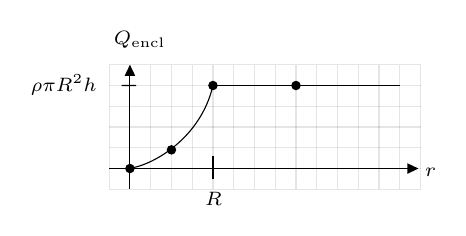
\begin{tikzpicture}[x=0.75pt,y=0.75pt,yscale=-1,xscale=1]
%uncomment if require: \path (0,96); %set diagram left start at 0, and has height of 96

%Shape: Grid [id:dp8393914292665905] 
\draw  [draw opacity=0] (49,20) -- (199,20) -- (199,80) -- (49,80) -- cycle ; \draw  [color={rgb, 255:red, 0; green, 0; blue, 0 }  ,draw opacity=0.1 ] (49,20) -- (49,80)(59,20) -- (59,80)(69,20) -- (69,80)(79,20) -- (79,80)(89,20) -- (89,80)(99,20) -- (99,80)(109,20) -- (109,80)(119,20) -- (119,80)(129,20) -- (129,80)(139,20) -- (139,80)(149,20) -- (149,80)(159,20) -- (159,80)(169,20) -- (169,80)(179,20) -- (179,80)(189,20) -- (189,80) ; \draw  [color={rgb, 255:red, 0; green, 0; blue, 0 }  ,draw opacity=0.1 ] (49,20) -- (199,20)(49,30) -- (199,30)(49,40) -- (199,40)(49,50) -- (199,50)(49,60) -- (199,60)(49,70) -- (199,70) ; \draw  [color={rgb, 255:red, 0; green, 0; blue, 0 }  ,draw opacity=0.1 ]  ;
%Straight Lines [id:da4895525400910108] 
\draw [color={rgb, 255:red, 0; green, 0; blue, 0 }  ,draw opacity=0.1 ]   (49,80) -- (199,80) ;
%Straight Lines [id:da2798886206430351] 
\draw [color={rgb, 255:red, 0; green, 0; blue, 0 }  ,draw opacity=0.1 ]   (199,80) -- (199,20) ;

%Straight Lines [id:da503236857304127] 
\draw    (59,23) -- (59,80) ;
\draw [shift={(59,20)}, rotate = 90] [fill={rgb, 255:red, 0; green, 0; blue, 0 }  ][line width=0.08]  [draw opacity=0] (5.36,-2.57) -- (0,0) -- (5.36,2.57) -- cycle    ;
%Straight Lines [id:da6760367650462902] 
\draw [color={rgb, 255:red, 0; green, 0; blue, 0 }  ,draw opacity=1 ]   (49,70) -- (195,70) ;
\draw [shift={(198,70)}, rotate = 180] [fill={rgb, 255:red, 0; green, 0; blue, 0 }  ,fill opacity=1 ][line width=0.08]  [draw opacity=0] (5.36,-2.57) -- (0,0) -- (5.36,2.57) -- cycle    ;
%Straight Lines [id:da052205339354011615] 
\draw    (99,64) -- (99,75) ;
%Shape: Circle [id:dp8635882652461428] 
\draw  [fill={rgb, 255:red, 0; green, 0; blue, 0 }  ,fill opacity=1 ] (77,61) .. controls (77,59.9) and (77.9,59) .. (79,59) .. controls (80.1,59) and (81,59.9) .. (81,61) .. controls (81,62.1) and (80.1,63) .. (79,63) .. controls (77.9,63) and (77,62.1) .. (77,61) -- cycle ;
%Shape: Circle [id:dp3042819121152154] 
\draw  [fill={rgb, 255:red, 0; green, 0; blue, 0 }  ,fill opacity=1 ] (57,70) .. controls (57,68.9) and (57.9,68) .. (59,68) .. controls (60.1,68) and (61,68.9) .. (61,70) .. controls (61,71.1) and (60.1,72) .. (59,72) .. controls (57.9,72) and (57,71.1) .. (57,70) -- cycle ;
%Shape: Circle [id:dp9607060849975249] 
\draw  [fill={rgb, 255:red, 0; green, 0; blue, 0 }  ,fill opacity=1 ] (97,30) .. controls (97,28.9) and (97.9,28) .. (99,28) .. controls (100.1,28) and (101,28.9) .. (101,30) .. controls (101,31.1) and (100.1,32) .. (99,32) .. controls (97.9,32) and (97,31.1) .. (97,30) -- cycle ;
%Shape: Circle [id:dp14150670214561645] 
\draw  [fill={rgb, 255:red, 0; green, 0; blue, 0 }  ,fill opacity=1 ] (137,30) .. controls (137,28.9) and (137.9,28) .. (139,28) .. controls (140.1,28) and (141,28.9) .. (141,30) .. controls (141,31.1) and (140.1,32) .. (139,32) .. controls (137.9,32) and (137,31.1) .. (137,30) -- cycle ;
%Curve Lines [id:da8502294977576981] 
\draw    (58,70) .. controls (69,69.01) and (93,56.01) .. (99,30) ;
%Straight Lines [id:da4198845796712818] 
\draw    (99,30) -- (189,30) ;
%Straight Lines [id:da3646909094624544] 
\draw    (62,30) -- (55,29.98) ;

% Text Node
\draw (50,2.4) node [anchor=north west][inner sep=0.75pt]  [font=\scriptsize]  {$Q_{\mathrm{encl}}$};
% Text Node
\draw (94,80.4) node [anchor=north west][inner sep=0.75pt]  [font=\scriptsize]  {$R$};
% Text Node
\draw (200,68.4) node [anchor=north west][inner sep=0.75pt]  [font=\scriptsize]  {$r$};
% Text Node
\draw (10,23.39) node [anchor=north west][inner sep=0.75pt]  [font=\scriptsize]  {$\rho \pi R^{2} h$};


\end{tikzpicture}

        \fi

\end{enumerate}

\newpage

\section{Spherical Shell}

A non--conducting spherical shell of radius $R$ has a charge of $+3Q$ uniformly distributed on its surface. Its cross--section is shown along with that of a Gaussian sphere with the same center and a radius $r$.



\tikzset{every picture/.style={line width=0.75pt}} %set default line width to 0.75pt        

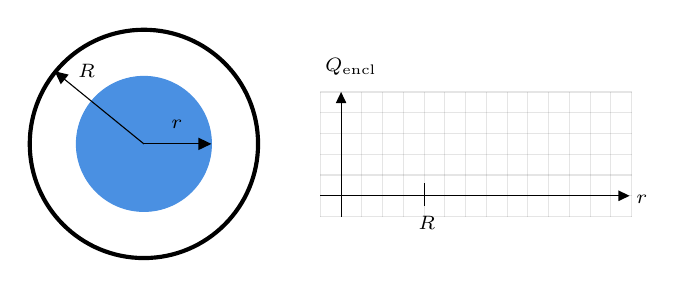
\begin{tikzpicture}[x=0.75pt,y=0.75pt,yscale=-1,xscale=1]
%uncomment if require: \path (0,128); %set diagram left start at 0, and has height of 128

%Shape: Circle [id:dp999367380646796] 
\draw  [color={rgb, 255:red, 74; green, 144; blue, 226 }  ,draw opacity=1 ][fill={rgb, 255:red, 74; green, 144; blue, 226 }  ,fill opacity=1 ] (32.49,65) .. controls (32.49,47.04) and (47.04,32.49) .. (65,32.49) .. controls (82.96,32.49) and (97.51,47.04) .. (97.51,65) .. controls (97.51,82.96) and (82.96,97.51) .. (65,97.51) .. controls (47.04,97.51) and (32.49,82.96) .. (32.49,65) -- cycle ;
%Shape: Circle [id:dp8804862003504208] 
\draw  [line width=1.5]  (10,65) .. controls (10,34.62) and (34.62,10) .. (65,10) .. controls (95.38,10) and (120,34.62) .. (120,65) .. controls (120,95.38) and (95.38,120) .. (65,120) .. controls (34.62,120) and (10,95.38) .. (10,65) -- cycle ;
%Straight Lines [id:da4163194444903606] 
\draw    (65,65) -- (94.51,65) ;
\draw [shift={(97.51,65)}, rotate = 180] [fill={rgb, 255:red, 0; green, 0; blue, 0 }  ][line width=0.08]  [draw opacity=0] (6.25,-3) -- (0,0) -- (6.25,3) -- cycle    ;
%Straight Lines [id:da7421060293052295] 
\draw    (65,65) -- (24.33,31.89) ;
\draw [shift={(22,30)}, rotate = 39.14] [fill={rgb, 255:red, 0; green, 0; blue, 0 }  ][line width=0.08]  [draw opacity=0] (6.25,-3) -- (0,0) -- (6.25,3) -- cycle    ;
%Shape: Grid [id:dp8281189839583585] 
\draw  [draw opacity=0] (150,40) -- (300,40) -- (300,100) -- (150,100) -- cycle ; \draw  [color={rgb, 255:red, 0; green, 0; blue, 0 }  ,draw opacity=0.1 ] (150,40) -- (150,100)(160,40) -- (160,100)(170,40) -- (170,100)(180,40) -- (180,100)(190,40) -- (190,100)(200,40) -- (200,100)(210,40) -- (210,100)(220,40) -- (220,100)(230,40) -- (230,100)(240,40) -- (240,100)(250,40) -- (250,100)(260,40) -- (260,100)(270,40) -- (270,100)(280,40) -- (280,100)(290,40) -- (290,100) ; \draw  [color={rgb, 255:red, 0; green, 0; blue, 0 }  ,draw opacity=0.1 ] (150,40) -- (300,40)(150,50) -- (300,50)(150,60) -- (300,60)(150,70) -- (300,70)(150,80) -- (300,80)(150,90) -- (300,90) ; \draw  [color={rgb, 255:red, 0; green, 0; blue, 0 }  ,draw opacity=0.1 ]  ;
%Straight Lines [id:da26407375789922694] 
\draw [color={rgb, 255:red, 0; green, 0; blue, 0 }  ,draw opacity=0.1 ]   (150,100) -- (300,100) ;
%Straight Lines [id:da8174118106915371] 
\draw [color={rgb, 255:red, 0; green, 0; blue, 0 }  ,draw opacity=0.1 ]   (300,100) -- (300,40) ;

%Straight Lines [id:da6047260798890028] 
\draw    (160,43) -- (160,100) ;
\draw [shift={(160,40)}, rotate = 90] [fill={rgb, 255:red, 0; green, 0; blue, 0 }  ][line width=0.08]  [draw opacity=0] (5.36,-2.57) -- (0,0) -- (5.36,2.57) -- cycle    ;
%Straight Lines [id:da9884061471215666] 
\draw [color={rgb, 255:red, 0; green, 0; blue, 0 }  ,draw opacity=1 ]   (150,90) -- (296,90) ;
\draw [shift={(299,90)}, rotate = 180] [fill={rgb, 255:red, 0; green, 0; blue, 0 }  ,fill opacity=1 ][line width=0.08]  [draw opacity=0] (5.36,-2.57) -- (0,0) -- (5.36,2.57) -- cycle    ;
%Straight Lines [id:da18701461337235648] 
\draw    (200,84) -- (200,95) ;

% Text Node
\draw (32,25.4) node [anchor=north west][inner sep=0.75pt]  [font=\scriptsize]  {$R$};
% Text Node
\draw (77,52.4) node [anchor=north west][inner sep=0.75pt]  [font=\scriptsize]  {$r$};
% Text Node
\draw (151,22.4) node [anchor=north west][inner sep=0.75pt]  [font=\scriptsize]  {$Q_{\mathrm{encl}}$};
% Text Node
\draw (196,98.4) node [anchor=north west][inner sep=0.75pt]  [font=\scriptsize]  {$R$};
% Text Node
\draw (301,88.4) node [anchor=north west][inner sep=0.75pt]  [font=\scriptsize]  {$r$};


\end{tikzpicture}


\begin{enumerate}

  \item Find the surface charge density on the sphere.

        \ifsolutions
          \textbf{Answer}: $\sigma = 3Q/4\pi R^2$
        \else
          \vskip 36.135pt
        \fi

  \item Find an equation for $Q_{\text{encl}}$ for $r<R$.

        \ifsolutions
          \textbf{Answer}: $Q_{\text{encl}}=0$
        \else
          \vskip 36.135pt
        \fi

  \item Find an equation for $Q_{\text{encl}}$ for $r>R$. Your equation should involve $\sigma$ and one or more of $R$ and $r$.

        \ifsolutions
          \textbf{Answer}: $Q_{\text{encl}}=\sigma 4\pi R^2$
        \else
          \vskip 36.135pt
        \fi

  \item Find the amount of charge enclosed in Gaussian sphere of radii $r=0$, $r=R/2$, $r=2R$, and $r=3R$.

        \ifsolutions
          \textbf{Answer}: $0, 0, \sigma 4 \pi R^2, \sigma 4\pi R^2$
        \else
          \vskip 36.135pt
        \fi

  \item Plot the four values of enclosed charge calculated above versus the radius of the Gaussian sphere. Then plot the equations found in parts 2. and 3 as a smooth line.

        \ifsolutions
          \textbf{Answer}: 
        
          

\tikzset{every picture/.style={line width=0.75pt}} %set default line width to 0.75pt        

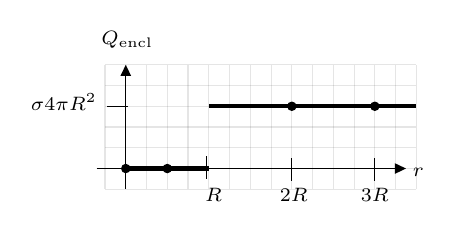
\begin{tikzpicture}[x=0.75pt,y=0.75pt,yscale=-1,xscale=1]
%uncomment if require: \path (0,94); %set diagram left start at 0, and has height of 94

%Shape: Grid [id:dp13795281087788713] 
\draw  [draw opacity=0] (40,20) -- (190,20) -- (190,80) -- (40,80) -- cycle ; \draw  [color={rgb, 255:red, 0; green, 0; blue, 0 }  ,draw opacity=0.1 ] (40,20) -- (40,80)(50,20) -- (50,80)(60,20) -- (60,80)(70,20) -- (70,80)(80,20) -- (80,80)(90,20) -- (90,80)(100,20) -- (100,80)(110,20) -- (110,80)(120,20) -- (120,80)(130,20) -- (130,80)(140,20) -- (140,80)(150,20) -- (150,80)(160,20) -- (160,80)(170,20) -- (170,80)(180,20) -- (180,80) ; \draw  [color={rgb, 255:red, 0; green, 0; blue, 0 }  ,draw opacity=0.1 ] (40,20) -- (190,20)(40,30) -- (190,30)(40,40) -- (190,40)(40,50) -- (190,50)(40,60) -- (190,60)(40,70) -- (190,70) ; \draw  [color={rgb, 255:red, 0; green, 0; blue, 0 }  ,draw opacity=0.1 ]  ;
%Straight Lines [id:da3072686147972945] 
\draw [color={rgb, 255:red, 0; green, 0; blue, 0 }  ,draw opacity=0.1 ]   (40,80) -- (190,80) ;
%Straight Lines [id:da8353384398529642] 
\draw [color={rgb, 255:red, 0; green, 0; blue, 0 }  ,draw opacity=0.1 ]   (190,80) -- (190,20) ;

%Straight Lines [id:da24510439010735996] 
\draw    (50,23) -- (50,80) ;
\draw [shift={(50,20)}, rotate = 90] [fill={rgb, 255:red, 0; green, 0; blue, 0 }  ][line width=0.08]  [draw opacity=0] (5.36,-2.57) -- (0,0) -- (5.36,2.57) -- cycle    ;
%Straight Lines [id:da33283373635543234] 
\draw [color={rgb, 255:red, 0; green, 0; blue, 0 }  ,draw opacity=1 ]   (36,70) -- (182,70) ;
\draw [shift={(185,70)}, rotate = 180] [fill={rgb, 255:red, 0; green, 0; blue, 0 }  ,fill opacity=1 ][line width=0.08]  [draw opacity=0] (5.36,-2.57) -- (0,0) -- (5.36,2.57) -- cycle    ;
%Shape: Circle [id:dp29102946866512713] 
\draw  [fill={rgb, 255:red, 0; green, 0; blue, 0 }  ,fill opacity=1 ] (48,70) .. controls (48,68.9) and (48.9,68) .. (50,68) .. controls (51.1,68) and (52,68.9) .. (52,70) .. controls (52,71.1) and (51.1,72) .. (50,72) .. controls (48.9,72) and (48,71.1) .. (48,70) -- cycle ;
%Shape: Circle [id:dp5421984891762992] 
\draw  [fill={rgb, 255:red, 0; green, 0; blue, 0 }  ,fill opacity=1 ] (68,70) .. controls (68,68.9) and (68.9,68) .. (70,68) .. controls (71.1,68) and (72,68.9) .. (72,70) .. controls (72,71.1) and (71.1,72) .. (70,72) .. controls (68.9,72) and (68,71.1) .. (68,70) -- cycle ;
%Shape: Circle [id:dp5084600757827353] 
\draw  [fill={rgb, 255:red, 0; green, 0; blue, 0 }  ,fill opacity=1 ] (128,40) .. controls (128,38.9) and (128.9,38) .. (130,38) .. controls (131.1,38) and (132,38.9) .. (132,40) .. controls (132,41.1) and (131.1,42) .. (130,42) .. controls (128.9,42) and (128,41.1) .. (128,40) -- cycle ;
%Shape: Circle [id:dp3027348841569153] 
\draw  [fill={rgb, 255:red, 0; green, 0; blue, 0 }  ,fill opacity=1 ] (168,40) .. controls (168,38.9) and (168.9,38) .. (170,38) .. controls (171.1,38) and (172,38.9) .. (172,40) .. controls (172,41.1) and (171.1,42) .. (170,42) .. controls (168.9,42) and (168,41.1) .. (168,40) -- cycle ;
%Straight Lines [id:da8794427134729941] 
\draw    (89,64) -- (89,75) ;
%Straight Lines [id:da7611457623879998] 
\draw    (41,40) -- (51,40) ;
%Straight Lines [id:da927553511481952] 
\draw [line width=1.5]    (90,40) -- (190,40) ;
%Straight Lines [id:da7934344879773034] 
\draw [line width=1.5]    (50,70) -- (90,70) ;
%Straight Lines [id:da5492533064104752] 
\draw    (130,65) -- (130,76) ;
%Straight Lines [id:da7242840398564145] 
\draw    (170,65) -- (170,76) ;

% Text Node
\draw (37,2.4) node [anchor=north west][inner sep=0.75pt]  [font=\scriptsize]  {$Q_{\mathrm{encl}}$};
% Text Node
\draw (87,78.4) node [anchor=north west][inner sep=0.75pt]  [font=\scriptsize]  {$R$};
% Text Node
\draw (3,32.4) node [anchor=north west][inner sep=0.75pt]  [font=\scriptsize]  {$\sigma 4\pi R^{2}$};
% Text Node
\draw (187,68.4) node [anchor=north west][inner sep=0.75pt]  [font=\scriptsize]  {$r$};
% Text Node
\draw (123,78.4) node [anchor=north west][inner sep=0.75pt]  [font=\scriptsize]  {$2R$};
% Text Node
\draw (162,78.4) node [anchor=north west][inner sep=0.75pt]  [font=\scriptsize]  {$3R$};


\end{tikzpicture}

        \fi

\end{enumerate}

\newpage

\section{Solid Sphere}

A non--conducting sphere of radius $R$ has a charge of $+3Q$ distributed uniformly throughout it. The cross--section of the sphere is shown along with a dashed line representing the surface of a Gaussian sphere, which has the same center as the charged sphere and a radius $r$.



\tikzset{every picture/.style={line width=0.75pt}} %set default line width to 0.75pt        

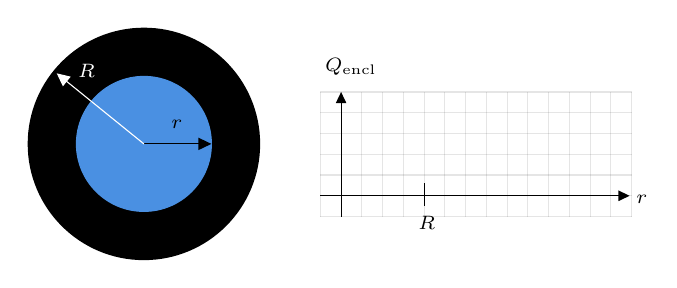
\begin{tikzpicture}[x=0.75pt,y=0.75pt,yscale=-1,xscale=1]
%uncomment if require: \path (0,128); %set diagram left start at 0, and has height of 128

%Shape: Circle [id:dp9766835204632047] 
\draw  [fill={rgb, 255:red, 0; green, 0; blue, 0 }  ,fill opacity=1 ][line width=1.5]  (10,65) .. controls (10,34.62) and (34.62,10) .. (65,10) .. controls (95.38,10) and (120,34.62) .. (120,65) .. controls (120,95.38) and (95.38,120) .. (65,120) .. controls (34.62,120) and (10,95.38) .. (10,65) -- cycle ;
%Shape: Circle [id:dp5025968278267186] 
\draw  [color={rgb, 255:red, 74; green, 144; blue, 226 }  ,draw opacity=1 ][fill={rgb, 255:red, 74; green, 144; blue, 226 }  ,fill opacity=1 ] (32.49,65) .. controls (32.49,47.04) and (47.04,32.49) .. (65,32.49) .. controls (82.96,32.49) and (97.51,47.04) .. (97.51,65) .. controls (97.51,82.96) and (82.96,97.51) .. (65,97.51) .. controls (47.04,97.51) and (32.49,82.96) .. (32.49,65) -- cycle ;
%Straight Lines [id:da579089752665406] 
\draw    (65,65) -- (94.51,65) ;
\draw [shift={(97.51,65)}, rotate = 180] [fill={rgb, 255:red, 0; green, 0; blue, 0 }  ][line width=0.08]  [draw opacity=0] (6.25,-3) -- (0,0) -- (6.25,3) -- cycle    ;
%Straight Lines [id:da3113687194658947] 
\draw [color={rgb, 255:red, 255; green, 255; blue, 255 }  ,draw opacity=1 ]   (65,65) -- (25.33,32.89) ;
\draw [shift={(23,31)}, rotate = 38.99] [fill={rgb, 255:red, 255; green, 255; blue, 255 }  ,fill opacity=1 ][line width=0.08]  [draw opacity=0] (6.25,-3) -- (0,0) -- (6.25,3) -- cycle    ;
%Shape: Grid [id:dp4072097255438287] 
\draw  [draw opacity=0] (150,40) -- (300,40) -- (300,100) -- (150,100) -- cycle ; \draw  [color={rgb, 255:red, 0; green, 0; blue, 0 }  ,draw opacity=0.1 ] (150,40) -- (150,100)(160,40) -- (160,100)(170,40) -- (170,100)(180,40) -- (180,100)(190,40) -- (190,100)(200,40) -- (200,100)(210,40) -- (210,100)(220,40) -- (220,100)(230,40) -- (230,100)(240,40) -- (240,100)(250,40) -- (250,100)(260,40) -- (260,100)(270,40) -- (270,100)(280,40) -- (280,100)(290,40) -- (290,100) ; \draw  [color={rgb, 255:red, 0; green, 0; blue, 0 }  ,draw opacity=0.1 ] (150,40) -- (300,40)(150,50) -- (300,50)(150,60) -- (300,60)(150,70) -- (300,70)(150,80) -- (300,80)(150,90) -- (300,90) ; \draw  [color={rgb, 255:red, 0; green, 0; blue, 0 }  ,draw opacity=0.1 ]  ;
%Straight Lines [id:da5916223647803596] 
\draw [color={rgb, 255:red, 0; green, 0; blue, 0 }  ,draw opacity=0.1 ]   (150,100) -- (300,100) ;
%Straight Lines [id:da028168436365389127] 
\draw [color={rgb, 255:red, 0; green, 0; blue, 0 }  ,draw opacity=0.1 ]   (300,100) -- (300,40) ;

%Straight Lines [id:da0004616455927557439] 
\draw    (160,43) -- (160,100) ;
\draw [shift={(160,40)}, rotate = 90] [fill={rgb, 255:red, 0; green, 0; blue, 0 }  ][line width=0.08]  [draw opacity=0] (5.36,-2.57) -- (0,0) -- (5.36,2.57) -- cycle    ;
%Straight Lines [id:da7260057623276042] 
\draw [color={rgb, 255:red, 0; green, 0; blue, 0 }  ,draw opacity=1 ]   (150,90) -- (296,90) ;
\draw [shift={(299,90)}, rotate = 180] [fill={rgb, 255:red, 0; green, 0; blue, 0 }  ,fill opacity=1 ][line width=0.08]  [draw opacity=0] (5.36,-2.57) -- (0,0) -- (5.36,2.57) -- cycle    ;
%Straight Lines [id:da5178691434385663] 
\draw    (200,84) -- (200,95) ;

% Text Node
\draw (32,25.4) node [anchor=north west][inner sep=0.75pt]  [font=\scriptsize,color={rgb, 255:red, 255; green, 255; blue, 255 }  ,opacity=1 ]  {$R$};
% Text Node
\draw (77,52.4) node [anchor=north west][inner sep=0.75pt]  [font=\scriptsize]  {$r$};
% Text Node
\draw (151,22.4) node [anchor=north west][inner sep=0.75pt]  [font=\scriptsize]  {$Q_{\mathrm{encl}}$};
% Text Node
\draw (196,98.4) node [anchor=north west][inner sep=0.75pt]  [font=\scriptsize]  {$R$};
% Text Node
\draw (301,88.4) node [anchor=north west][inner sep=0.75pt]  [font=\scriptsize]  {$r$};


\end{tikzpicture}


\begin{enumerate}

  \item Find the charged sphere's volume charge density, $\rho$.

        \ifsolutions
          \textbf{Answer}: $\ds \rho=3Q/[(4/3)\pi R^3]$
        \else
          \vskip 36.135pt
        \fi

  \item Find an equation for $Q_{\text{encl}}$ for $r<R$. Your answer should involve $\rho$ and one or more of $r$ and $R$.

        \ifsolutions
          \textbf{Answer}: For $r \le R$, $Q_{\text{encl}}=\rho [(4/3)\pi r^3]$
        \else
          \vskip 36.135pt
        \fi

  \item Find an equation for $Q_{\text{encl}}$ for $r>R$. Your answer should involve $\rho$ and one or more of $r$ and $R$.

        \ifsolutions
          \textbf{Answer}: For $r \ge R$,  $Q_{\text{encl}}=\rho [(4/3)\pi R^3]$, which is independent of $r$.
        \else
          \vskip 36.135pt
        \fi

  \item Find the amount of charge enclosed in Gaussian sphere of radii $r=0$, $r=R/2$, $r=R$, and $r=2R$.

        \ifsolutions
          \textbf{Answer}: $0, (1/8)\rho (4/3)\pi R^3, \rho(4/3)\pi R^3, \rho(4/3)\pi R^3$
        \else
          \vskip 36.135pt
        \fi

  \item Plot the four values of enclosed charge calculated above versus the radius of the Gaussian sphere. Then plot the equations found in parts 2. and 3 as a smooth line.

        \ifsolutions
          

\tikzset{every picture/.style={line width=0.75pt}} %set default line width to 0.75pt        

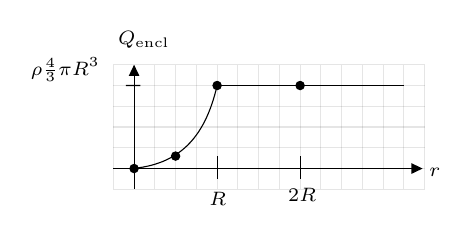
\begin{tikzpicture}[x=0.75pt,y=0.75pt,yscale=-1,xscale=1]
%uncomment if require: \path (0,96); %set diagram left start at 0, and has height of 96

%Shape: Grid [id:dp6010151406802797] 
\draw  [draw opacity=0] (50,20) -- (200,20) -- (200,80) -- (50,80) -- cycle ; \draw  [color={rgb, 255:red, 0; green, 0; blue, 0 }  ,draw opacity=0.1 ] (50,20) -- (50,80)(60,20) -- (60,80)(70,20) -- (70,80)(80,20) -- (80,80)(90,20) -- (90,80)(100,20) -- (100,80)(110,20) -- (110,80)(120,20) -- (120,80)(130,20) -- (130,80)(140,20) -- (140,80)(150,20) -- (150,80)(160,20) -- (160,80)(170,20) -- (170,80)(180,20) -- (180,80)(190,20) -- (190,80) ; \draw  [color={rgb, 255:red, 0; green, 0; blue, 0 }  ,draw opacity=0.1 ] (50,20) -- (200,20)(50,30) -- (200,30)(50,40) -- (200,40)(50,50) -- (200,50)(50,60) -- (200,60)(50,70) -- (200,70) ; \draw  [color={rgb, 255:red, 0; green, 0; blue, 0 }  ,draw opacity=0.1 ]  ;
%Straight Lines [id:da4038653043597724] 
\draw [color={rgb, 255:red, 0; green, 0; blue, 0 }  ,draw opacity=0.1 ]   (50,80) -- (200,80) ;
%Straight Lines [id:da6738316203697128] 
\draw [color={rgb, 255:red, 0; green, 0; blue, 0 }  ,draw opacity=0.1 ]   (200,80) -- (200,20) ;

%Straight Lines [id:da9172563707447259] 
\draw    (60,23) -- (60,80) ;
\draw [shift={(60,20)}, rotate = 90] [fill={rgb, 255:red, 0; green, 0; blue, 0 }  ][line width=0.08]  [draw opacity=0] (5.36,-2.57) -- (0,0) -- (5.36,2.57) -- cycle    ;
%Straight Lines [id:da23724680902794404] 
\draw [color={rgb, 255:red, 0; green, 0; blue, 0 }  ,draw opacity=1 ]   (50,70) -- (196,70) ;
\draw [shift={(199,70)}, rotate = 180] [fill={rgb, 255:red, 0; green, 0; blue, 0 }  ,fill opacity=1 ][line width=0.08]  [draw opacity=0] (5.36,-2.57) -- (0,0) -- (5.36,2.57) -- cycle    ;
%Straight Lines [id:da23155879097316978] 
\draw    (100,64) -- (100,75) ;
%Shape: Circle [id:dp6274356429435639] 
\draw  [fill={rgb, 255:red, 0; green, 0; blue, 0 }  ,fill opacity=1 ] (78,64) .. controls (78,62.9) and (78.9,62) .. (80,62) .. controls (81.1,62) and (82,62.9) .. (82,64) .. controls (82,65.1) and (81.1,66) .. (80,66) .. controls (78.9,66) and (78,65.1) .. (78,64) -- cycle ;
%Shape: Circle [id:dp22257979360119906] 
\draw  [fill={rgb, 255:red, 0; green, 0; blue, 0 }  ,fill opacity=1 ] (58,70) .. controls (58,68.9) and (58.9,68) .. (60,68) .. controls (61.1,68) and (62,68.9) .. (62,70) .. controls (62,71.1) and (61.1,72) .. (60,72) .. controls (58.9,72) and (58,71.1) .. (58,70) -- cycle ;
%Shape: Circle [id:dp0656010548956738] 
\draw  [fill={rgb, 255:red, 0; green, 0; blue, 0 }  ,fill opacity=1 ] (98,30) .. controls (98,28.9) and (98.9,28) .. (100,28) .. controls (101.1,28) and (102,28.9) .. (102,30) .. controls (102,31.1) and (101.1,32) .. (100,32) .. controls (98.9,32) and (98,31.1) .. (98,30) -- cycle ;
%Shape: Circle [id:dp3642837356026165] 
\draw  [fill={rgb, 255:red, 0; green, 0; blue, 0 }  ,fill opacity=1 ] (138,30) .. controls (138,28.9) and (138.9,28) .. (140,28) .. controls (141.1,28) and (142,28.9) .. (142,30) .. controls (142,31.1) and (141.1,32) .. (140,32) .. controls (138.9,32) and (138,31.1) .. (138,30) -- cycle ;
%Curve Lines [id:da010603345574577983] 
\draw    (59,70) .. controls (81.07,68.03) and (94,56.01) .. (100,30) ;
%Straight Lines [id:da5454319512174814] 
\draw    (100,30) -- (190,30) ;
%Straight Lines [id:da6851517141073331] 
\draw    (63,30) -- (56,29.98) ;
%Straight Lines [id:da9064673163485206] 
\draw    (140,64) -- (140,75) ;

% Text Node
\draw (51,2.4) node [anchor=north west][inner sep=0.75pt]  [font=\scriptsize]  {$Q_{\mathrm{encl}}$};
% Text Node
\draw (95,80.4) node [anchor=north west][inner sep=0.75pt]  [font=\scriptsize]  {$R$};
% Text Node
\draw (201,68.4) node [anchor=north west][inner sep=0.75pt]  [font=\scriptsize]  {$r$};
% Text Node
\draw (9,15.4) node [anchor=north west][inner sep=0.75pt]  [font=\scriptsize]  {$\rho \frac{4}{3} \pi R^{3}$};
% Text Node
\draw (133,78.4) node [anchor=north west][inner sep=0.75pt]  [font=\scriptsize]  {$2R$};


\end{tikzpicture}

        \fi

\end{enumerate}

\newpage

\section{Large Sheet}



\tikzset{every picture/.style={line width=0.75pt}} %set default line width to 0.75pt        

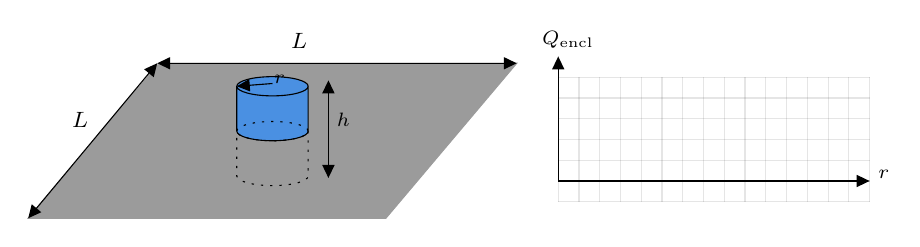
\begin{tikzpicture}[x=0.75pt,y=0.75pt,yscale=-1,xscale=1]
%uncomment if require: \path (0,121); %set diagram left start at 0, and has height of 121

%Shape: Rectangle [id:dp4651784594834052] 
\draw  [color={rgb, 255:red, 155; green, 155; blue, 155 }  ,draw opacity=1 ][fill={rgb, 255:red, 155; green, 155; blue, 155 }  ,fill opacity=1 ] (67.67,33.28) -- (240,33.28) -- (176.97,107.93) -- (4.64,107.93) -- cycle ;
%Shape: Can [id:dp7305061547019078] 
\draw  [fill={rgb, 255:red, 74; green, 144; blue, 226 }  ,fill opacity=1 ] (139.51,44.36) -- (139.51,65.97) .. controls (139.51,68.53) and (131.82,70.61) .. (122.32,70.61) .. controls (112.83,70.61) and (105.13,68.53) .. (105.13,65.97) -- (105.13,44.36) .. controls (105.13,41.8) and (112.83,39.73) .. (122.32,39.73) .. controls (131.82,39.73) and (139.51,41.8) .. (139.51,44.36) .. controls (139.51,46.92) and (131.82,48.99) .. (122.32,48.99) .. controls (112.83,48.99) and (105.13,46.92) .. (105.13,44.36) ;
%Shape: Can [id:dp15610817211700656] 
\draw  [dash pattern={on 0.84pt off 2.51pt}] (139.51,65.97) -- (139.51,87.59) .. controls (139.51,90.14) and (131.82,92.22) .. (122.32,92.22) .. controls (112.83,92.22) and (105.13,90.14) .. (105.13,87.59) -- (105.13,65.97) .. controls (105.13,63.42) and (112.83,61.34) .. (122.32,61.34) .. controls (131.82,61.34) and (139.51,63.42) .. (139.51,65.97) .. controls (139.51,68.53) and (131.82,70.61) .. (122.32,70.61) .. controls (112.83,70.61) and (105.13,68.53) .. (105.13,65.97) ;
%Straight Lines [id:da29104893461111936] 
\draw    (122.32,43.03) -- (108.12,44.13) ;
\draw [shift={(105.13,44.36)}, rotate = 355.57] [fill={rgb, 255:red, 0; green, 0; blue, 0 }  ][line width=0.08]  [draw opacity=0] (6.25,-3) -- (0,0) -- (6.25,3) -- cycle    ;
%Straight Lines [id:da89111533876494] 
\draw    (149.27,44.53) -- (149.27,85.54) ;
\draw [shift={(149.27,88.54)}, rotate = 270] [fill={rgb, 255:red, 0; green, 0; blue, 0 }  ][line width=0.08]  [draw opacity=0] (6.25,-3) -- (0,0) -- (6.25,3) -- cycle    ;
\draw [shift={(149.27,41.53)}, rotate = 90] [fill={rgb, 255:red, 0; green, 0; blue, 0 }  ][line width=0.08]  [draw opacity=0] (6.25,-3) -- (0,0) -- (6.25,3) -- cycle    ;
%Straight Lines [id:da8160819861971584] 
\draw    (6.56,105.62) -- (64.88,35.59) ;
\draw [shift={(66.8,33.28)}, rotate = 129.78] [fill={rgb, 255:red, 0; green, 0; blue, 0 }  ][line width=0.08]  [draw opacity=0] (6.25,-3) -- (0,0) -- (6.25,3) -- cycle    ;
\draw [shift={(4.64,107.93)}, rotate = 309.78] [fill={rgb, 255:red, 0; green, 0; blue, 0 }  ][line width=0.08]  [draw opacity=0] (6.25,-3) -- (0,0) -- (6.25,3) -- cycle    ;
%Straight Lines [id:da028742244954956364] 
\draw    (69.8,33.28) -- (237,33.28) ;
\draw [shift={(240,33.28)}, rotate = 180] [fill={rgb, 255:red, 0; green, 0; blue, 0 }  ][line width=0.08]  [draw opacity=0] (6.25,-3) -- (0,0) -- (6.25,3) -- cycle    ;
\draw [shift={(66.8,33.28)}, rotate = 0] [fill={rgb, 255:red, 0; green, 0; blue, 0 }  ][line width=0.08]  [draw opacity=0] (6.25,-3) -- (0,0) -- (6.25,3) -- cycle    ;
%Shape: Grid [id:dp2121744369829328] 
\draw  [draw opacity=0] (260,40) -- (410,40) -- (410,100) -- (260,100) -- cycle ; \draw  [color={rgb, 255:red, 0; green, 0; blue, 0 }  ,draw opacity=0.1 ] (260,40) -- (260,100)(270,40) -- (270,100)(280,40) -- (280,100)(290,40) -- (290,100)(300,40) -- (300,100)(310,40) -- (310,100)(320,40) -- (320,100)(330,40) -- (330,100)(340,40) -- (340,100)(350,40) -- (350,100)(360,40) -- (360,100)(370,40) -- (370,100)(380,40) -- (380,100)(390,40) -- (390,100)(400,40) -- (400,100) ; \draw  [color={rgb, 255:red, 0; green, 0; blue, 0 }  ,draw opacity=0.1 ] (260,40) -- (410,40)(260,50) -- (410,50)(260,60) -- (410,60)(260,70) -- (410,70)(260,80) -- (410,80)(260,90) -- (410,90) ; \draw  [color={rgb, 255:red, 0; green, 0; blue, 0 }  ,draw opacity=0.1 ]  ;
%Straight Lines [id:da07530414796534357] 
\draw [color={rgb, 255:red, 0; green, 0; blue, 0 }  ,draw opacity=0.1 ]   (260,100) -- (410,100) ;
%Straight Lines [id:da41747836013746364] 
\draw [color={rgb, 255:red, 0; green, 0; blue, 0 }  ,draw opacity=0.1 ]   (410,100) -- (410,40) ;

%Straight Lines [id:da2324027134572988] 
\draw    (260,33) -- (260,90) ;
\draw [shift={(260,30)}, rotate = 90] [fill={rgb, 255:red, 0; green, 0; blue, 0 }  ][line width=0.08]  [draw opacity=0] (6.25,-3) -- (0,0) -- (6.25,3) -- cycle    ;
%Straight Lines [id:da11247137813852492] 
\draw    (260,90) -- (407,90) ;
\draw [shift={(410,90)}, rotate = 180] [fill={rgb, 255:red, 0; green, 0; blue, 0 }  ][line width=0.08]  [draw opacity=0] (6.25,-3) -- (0,0) -- (6.25,3) -- cycle    ;

% Text Node
\draw (121.83,37.76) node [anchor=north west][inner sep=0.75pt]  [font=\scriptsize]  {$r$};
% Text Node
\draw (152.06,55.9) node [anchor=north west][inner sep=0.75pt]  [font=\scriptsize]  {$h$};
% Text Node
\draw (130.08,17.79) node [anchor=north west][inner sep=0.75pt]  [font=\footnotesize]  {$L$};
% Text Node
\draw (24.51,55.73) node [anchor=north west][inner sep=0.75pt]  [font=\footnotesize]  {$L$};
% Text Node
\draw (251,16.4) node [anchor=north west][inner sep=0.75pt]  [font=\scriptsize]  {$Q\mathrm{_{encl}}$};
% Text Node
\draw (413,83.4) node [anchor=north west][inner sep=0.75pt]  [font=\scriptsize]  {$r$};


\end{tikzpicture}


A non--conducting square sheet with side length $L$ has a charge of $+3Q$ distributed uniformly on it. The Gaussian cylinder has a height $h$ and radius $r$, and half of it is above the sheet.

\begin{enumerate}

  \item Find the surface charge density, $\sigma$, on the sheet.

        \ifsolutions
          \textbf{Answer}: $\sigma=3Q/L^2$
        \else
          \vskip 36.135pt
        \fi

  \item Find an equation for $Q_{\text{encl}}$ for $r<L$. Your answer should involve $\sigma$ and one or more of $r$, $h$, and $L$. (In Gauss's law problems, $L$ is much larger than $r$, so we do not need to consider $r > L$.)

        \ifsolutions
          \textbf{Answer}: $Q_{\text{encl}}=\sigma \pi r^2$.
        \else
          \vskip 36.135pt
        \fi

  \item Plot the enclosed charge calculated above versus the radius of the Gaussian cylinder.

        \ifsolutions
          

\tikzset{every picture/.style={line width=0.75pt}} %set default line width to 0.75pt        

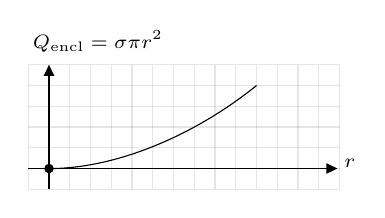
\begin{tikzpicture}[x=0.75pt,y=0.75pt,yscale=-1,xscale=1]
%uncomment if require: \path (0,87); %set diagram left start at 0, and has height of 87

%Shape: Grid [id:dp036989104826425034] 
\draw  [draw opacity=0] (10,20) -- (160,20) -- (160,80) -- (10,80) -- cycle ; \draw  [color={rgb, 255:red, 0; green, 0; blue, 0 }  ,draw opacity=0.1 ] (10,20) -- (10,80)(20,20) -- (20,80)(30,20) -- (30,80)(40,20) -- (40,80)(50,20) -- (50,80)(60,20) -- (60,80)(70,20) -- (70,80)(80,20) -- (80,80)(90,20) -- (90,80)(100,20) -- (100,80)(110,20) -- (110,80)(120,20) -- (120,80)(130,20) -- (130,80)(140,20) -- (140,80)(150,20) -- (150,80) ; \draw  [color={rgb, 255:red, 0; green, 0; blue, 0 }  ,draw opacity=0.1 ] (10,20) -- (160,20)(10,30) -- (160,30)(10,40) -- (160,40)(10,50) -- (160,50)(10,60) -- (160,60)(10,70) -- (160,70) ; \draw  [color={rgb, 255:red, 0; green, 0; blue, 0 }  ,draw opacity=0.1 ]  ;
%Straight Lines [id:da9110657930117563] 
\draw [color={rgb, 255:red, 0; green, 0; blue, 0 }  ,draw opacity=0.1 ]   (10,80) -- (160,80) ;
%Straight Lines [id:da9537398910246793] 
\draw [color={rgb, 255:red, 0; green, 0; blue, 0 }  ,draw opacity=0.1 ]   (160,80) -- (160,20) ;

%Straight Lines [id:da8928276270226045] 
\draw    (20,23) -- (20,80) ;
\draw [shift={(20,20)}, rotate = 90] [fill={rgb, 255:red, 0; green, 0; blue, 0 }  ][line width=0.08]  [draw opacity=0] (5.36,-2.57) -- (0,0) -- (5.36,2.57) -- cycle    ;
%Straight Lines [id:da21991350173696778] 
\draw [color={rgb, 255:red, 0; green, 0; blue, 0 }  ,draw opacity=1 ]   (10,70) -- (156,70) ;
\draw [shift={(159,70)}, rotate = 180] [fill={rgb, 255:red, 0; green, 0; blue, 0 }  ,fill opacity=1 ][line width=0.08]  [draw opacity=0] (5.36,-2.57) -- (0,0) -- (5.36,2.57) -- cycle    ;
%Shape: Circle [id:dp3990152675244536] 
\draw  [fill={rgb, 255:red, 0; green, 0; blue, 0 }  ,fill opacity=1 ] (18,70) .. controls (18,68.9) and (18.9,68) .. (20,68) .. controls (21.1,68) and (22,68.9) .. (22,70) .. controls (22,71.1) and (21.1,72) .. (20,72) .. controls (18.9,72) and (18,71.1) .. (18,70) -- cycle ;
%Curve Lines [id:da0637629892146847] 
\draw    (22,70) .. controls (54,69.43) and (91,53.43) .. (120,30) ;

% Text Node
\draw (11,2.4) node [anchor=north west][inner sep=0.75pt]  [font=\scriptsize]  {$Q_{\mathrm{encl}} =\sigma \pi r^{2}$};
% Text Node
\draw (161,64.4) node [anchor=north west][inner sep=0.75pt]  [font=\scriptsize]  {$r$};


\end{tikzpicture}

        \fi

\end{enumerate}

\end{document}